\chapter{线性回归}

为了让上面的房屋示例更有趣,不妨考虑一个更为丰富的数据集。除了居住面积外,该数据集还包括了每栋房屋的卧室数量:

\begin{table}[H]
    \centering
    \begin{tabular}{c|c|c}
        居住面积 (平方英尺) & 卧室数 & 价格 (1000\$) \\
        \hline
        2104 & 3 & 400 \\
        1600 & 3 & 330 \\
        2400 & 3 & 369 \\
        1416 & 2 & 232 \\
        3000 & 4 & 540 \\
        $\vdots$ & $\vdots$ & $\vdots$
    \end{tabular}
    \label{tab:house_example2}
\end{table}

此处,$x$ 是 $\mathbb{R}^2$ 中的二维向量。对于训练集中第 $i$ 栋房屋,$x_1^{(i)}$ 是其居住面积,而 $x_2^{(i)}$ 是其卧室数量。(在设计学习问题时,特征的选择通常取决于你的具体需求。例如,在收集波特兰的房屋数据时,除了居住面积和卧室数量,还可以考虑纳入壁炉、浴室数量等其他特征。关于特征选择的深入讨论将在后续展开,目前先基于当前给定的两个特征进行分析。)

在进行监督学习时,需要明确如何在计算机中表示假设函数 $h$。不妨先尝试用 $x$ 的线性函数来近似 $y$:

\[
    h_\theta(x) = \theta_0 + \theta_1x_1 + \theta_2x_2
\]
在此处,$\theta_i$ 是该模型的\textbf{参数 (parameters)},亦称\textbf{权重 (weights)}。它们参数化了从特征空间 $\mathcal{X}$ 到目标空间 $\mathcal{Y}$ 的线性函数。在不引起混淆的前提下,可以省略 $h_\theta(x)$ 中的下标 $\theta$,直接写作 $h(x)$。为了进一步简化表示,我们引入约定:令 $x_0 = 1$。这个 $x_0$ 对应的系数 $\theta_0$ 通常被称为\textbf{截距项 (intercept term)}。这样就有

\[
    h(x) = \sum_{i=0}^d \theta_i x_i = \theta^T x,
\]
其中 $\theta$ 和 $x$ 视为向量,而 $d$ 则是输入变量的数量 (不计入 $x_0$)。

现在,对于给定的训练集,我们应该如何选择或学习参数 $\theta$ 呢?一个直观且合理的方法是,使假设函数 $h(x)$ 对于训练样本的输出 $h_\theta(x^{(i)})$ 尽可能地接近其对应的真实值 $y^{(i)}$。为了形式化地表述这个接近程度,我们定义一个函数,用于衡量对于任意给定的参数值 $\theta$,预测值 $h_\theta(x^{(i)})$ 与实际值 $y^{(i)}$ 之间的差异。这个函数被称为\textbf{代价函数 (cost function)}:

\[
    J(\theta) = \frac{1}{2} \sum_{i=1}^n (h_\theta(x^{(i)}) - y^{(i)})^2.
\]

熟悉线性回归的读者可能会发现,此处定义的函数即为\textbf{普通最小二乘 (ordinary least squares)} 回归模型所使用的最小二乘代价函数。但本讲义不要求读者具备相关背景知识,后文将对此进行详细阐述,并最终指出这仅是更广泛算法族中的一个特例。


\section{最小均方算法}

我们的目标是找到能够最小化代价函数 $J(\theta)$ 的参数 $\theta$。为此,我们可以考虑一种搜索算法:该算法从对 $\theta$ 的某个“初始猜测”开始,然后不断地调整 $\theta$ 的值,使其沿着使 $J(\theta)$ 减小的方向移动,直到最终收敛到最小化 $J(\theta)$ 的 $\theta$ 值。具体而言,我们考虑使用\textbf{梯度下降 (gradient descent)} 算法。该算法从某个初始的 $\theta$ 值开始,并重复执行以下更新步骤:

\[
    \theta_j := \theta_j - \alpha \frac{\partial}{\partial\theta_j} J(\theta).
\]
(上述更新操作同时应用于 $j = 0, \dots, d$ 的所有参数 $\theta_j$。)这里的 $\alpha$ 被称为\textbf{学习率 (learning rate)}。这是一种非常自然的算法:它每一步都沿着代价函数 $J$ 下降最快的方向进行更新。

为了实现上述算法,需要计算公式右侧的偏导数项。可以先考虑只有一个训练样本 $(x, y)$ 的情况,这样就可以暂时忽略代价函数 $J$ 定义中的求和操作。在这种情况下,偏导数计算如下:

\[
    \begin{aligned}
    \frac{\partial}{\partial\theta_j} J(\theta) &= \frac{\partial}{\partial\theta_j} \frac{1}{2} (h_\theta(x) - y)^2 \\
    &= 2 \cdot \frac{1}{2} (h_\theta(x) - y) \cdot \frac{\partial}{\partial\theta_j} (h_\theta(x) - y) \\
    &= (h_\theta(x) - y) \cdot \frac{\partial}{\partial\theta_j} \left( \sum_{i=0}^d \theta_i x_i - y \right) \\
    &= (h_\theta(x) - y) x_j
    \end{aligned}
\]

上式给出了针对单个训练样本的更新规则\footnote{符号 “$a := b$” 用于表示(计算机程序中的)一个操作,其中变量 $a$ 的值被设置为 $b$。换句话说,这个操作用 $b$ 的值覆盖了 $a$ 的值。反之,如果需要断言 $a$ 的值等于 $b$ 的值,会写作 “$a = b$”。}:

\[
    \theta_j := \theta_j + \alpha (y^{(i)} - h_\theta(x^{(i)})) x_j^{(i)}.
\]
这个规则被称为\textbf{最小均方 (Least mean squares, LMS)} 更新规则,也称为 \textbf{Widrow-Hoff} 学习规则。该规则具有一些自然而直观的特性。例如,更新的幅度与\textbf{误差 (error)} 项 $(y^{(i)} - h_\theta(x^{(i)}))$ 成正比;因此,如果对于一个训练样本,其预测值几乎等于 $y^{(i)}$ 的实际值,那么参数就几乎不需要调整;反之,如果预测的 $h_\theta(x^{(i)})$ 有很大的误差 (即与 $y^{(i)}$ 相差甚远),则需要对参数进行更大的调整。

所推导的 LMS 规则是针对只有一个训练样本的情况。要将其应用于包含多个样本的训练集,有两种常见的方法。第一种方法是将算法修改为以下形式:

\vspace{0.5em}
重复直到收敛 \{
\begin{equation}
    \theta_j := \theta_j + \alpha \sum_{i=1}^n (y^{(i)} - h_\theta(x^{(i)})) x_j^{(i)}, \text{(对于每个 } j) \label{eq:1.1}
\end{equation}
\indent\}
\vspace{0.5em}

将逐位置的更新向量化到 $\theta$,可以稍微简化 \eqref{eq:1.1}:

\[
    \theta := \theta + \alpha \sum_{i=1}^n (y^{(i)} - h_\theta(x^{(i)})) x^{(i)}
\]

读者不难验证,上述更新规则中求和项所表示的量,恰好对应于我们先前定义的成本函数的偏导数 $\partial J(\theta) / \partial \theta_j$。因此,这个更新规则实际上就是在原始成本函数 $J$ 上进行梯度下降。这种方法在每一步都利用了整个训练集的所有样本,因此被称为\textbf{批量梯度下降 (batch gradient descent)}。值得注意的是,尽管梯度下降算法在一般情况下可能收敛到局部最优解,但对于我们这里的线性回归问题,其优化目标函数 $J$ 具有良好的性质:它是一个凸二次函数。这意味着它只有一个全局最小值,没有其他局部最优解。因此,在合适的学习率 $\alpha$ 下,梯度下降算法能够保证收敛到全局最优解。下面是一个用梯度下降最小化一个二次函数的图例。

\begin{figure}[H]
    \centering
    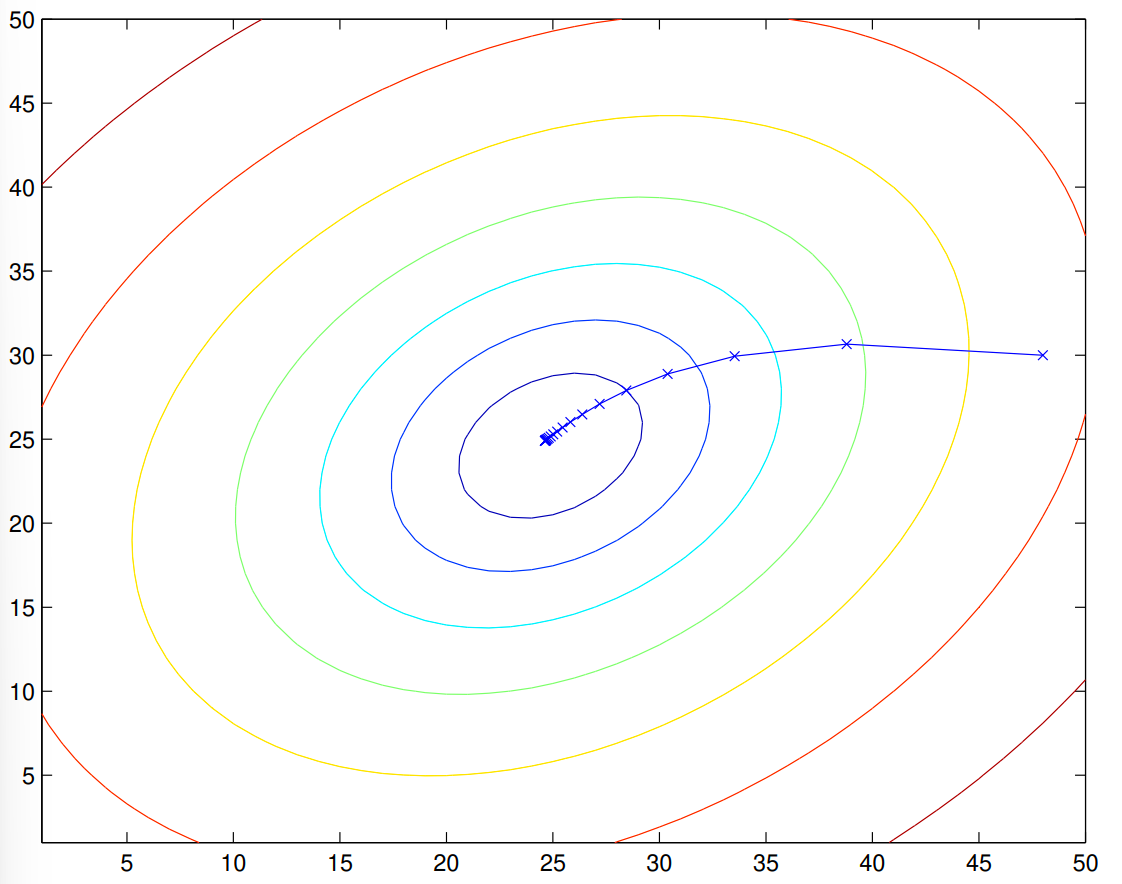
\includegraphics[width=0.5\linewidth]{figs/gradient_descent_trajectory.png}
    \label{fig:gradient_descent_trajectory}
\end{figure}
上面的椭圆是二次函数的等高线。图中还显示了梯度下降的轨迹,其初始化参数是 (48,30),而由直线连接的叉号 $\text{x}$ 则是梯度下降所经过的一系列参数 $\theta$ 值。

在之前的数据集上应用批量梯度下降算法来拟合参数 $\theta$,以学习根据居住面积预测房价的函数,最终得到的参数值为 $\theta_0 = 71.27$ 和 $\theta_1 = 0.1345$。将学习到的函数 $h_\theta(x)$,作为输入变量 $x$(表示居住面积)的函数,与训练数据一同绘制,结果如下图所示:

\begin{figure}[H]
    \centering
    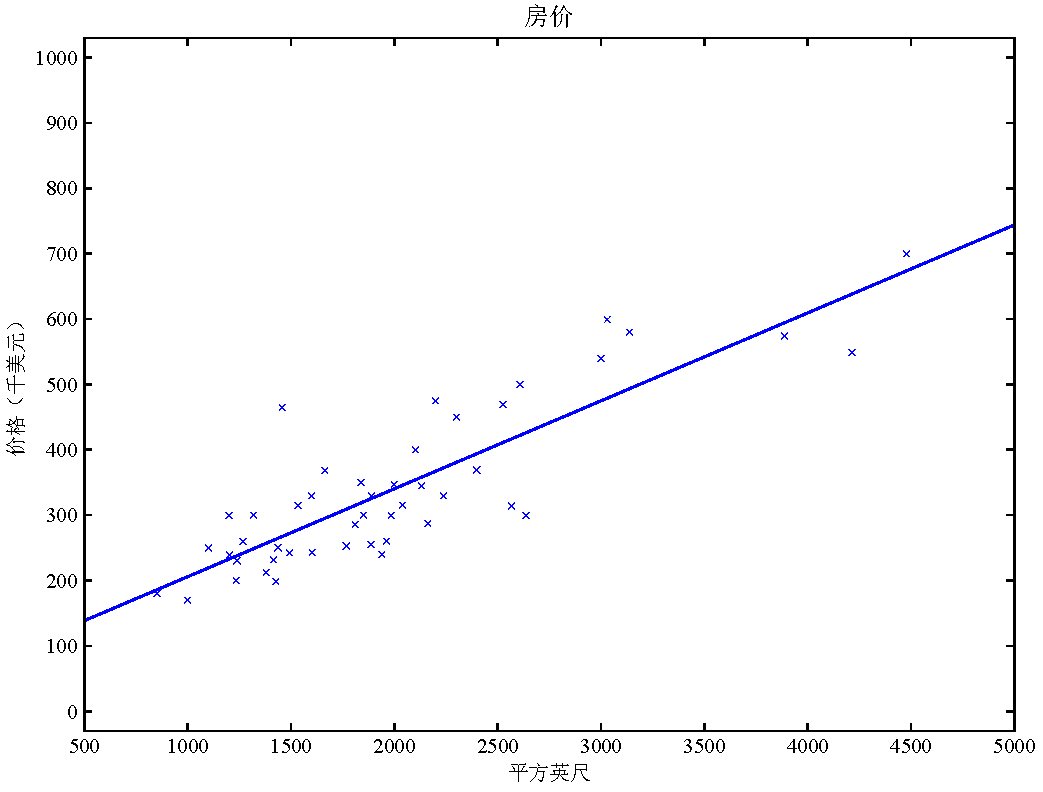
\includegraphics[width=0.5\linewidth]{figs/house_dataset_plot2.pdf}
\end{figure}
如果把卧室数量也当作输入特征,最终得到的参数值为 $\theta_0 = 89.60, \theta_1 = 0.1392, \theta_2 = -8.738$。

上述结果是通过批量梯度下降算法得到的。除此之外,还有一种很好的替代算法:

\vspace{0.5em}
循环 \{

$\quad\quad$对于 $i = 1$ 到 $n$,\{

\begin{equation}
    \theta_j := \theta_j + \alpha (y^{(i)} - h_\theta(x^{(i)})) x_j^{(i)}, \text{(对于每个 } j) \label{eq:1.2}
\end{equation}

$\quad\quad$\}

\indent\}
\vspace{0.5em}

将逐位置的更新向量化到 $\theta$,可以稍微简化 \eqref{eq:1.2}:

\[
    \theta := \theta + \alpha (y^{(i)} - h_\theta(x^{(i)})) x^{(i)}
\]

这种算法会重复遍历训练集,每次遇到一个训练样本时,仅针对该单个样本计算误差梯度并更新参数。这种方法被称为\textbf{随机梯度下降 (stochastic gradient descent)},有时也称为\textbf{增量梯度下降 (incremental gradient descent)}。与批量梯度下降不同,批量梯度下降在执行单次更新前需要扫描整个训练集(当训练集规模 $n$ 很大时,这是一项昂贵的操作),而随机梯度下降可以立即开始并对每个样本都取得进展。通常情况下,随机梯度下降能更快地使参数 $\theta$ “接近”最小值。然而,需要注意的是,它可能不会完全“收敛”到最小值,参数 $\theta$ 可能会在目标函数 $J(\theta)$ 的最小值附近持续振荡。但在实际应用中,接近最小值的大多数值都足以作为真实最小值的良好近似\footnote{通过在算法运行过程中缓慢地减小学习率 $\alpha$ 至零,可以确保参数收敛到全局最小值,而不仅仅是在最小值附近振荡。} 。因此,特别是在训练集很大时,通常更倾向于使用随机梯度下降而非批量梯度下降。


\section{正规方程}

梯度下降提供了一种最小化目标函数 $J$ 的迭代方法。接下来,我们将探讨另一种无需迭代的最小化 $J$ 的方法。具体而言,我们将通过明确地计算 $J$ 关于每个参数 $\theta_j$ 的偏导数,并将这些导数置为零来求解最小值。为了避免繁琐的代数运算和大量的导数矩阵书写,我们将在下文引入一些矩阵微积分的记号。

\subsection{矩阵导数}

对于一个将 $n \times d$ 矩阵映射到实数的函数 $f: \mathbb{R}^{n \times d} \mapsto \mathbb{R}$,我们定义 $f$ 对 $A$ 的导数:

\[
    \nabla_A f(A) = \begin{bmatrix} 
        &\frac{\partial f}{\partial A_{11}} & \cdots & \frac{\partial f}{\partial A_{1d}} & \\ 
        &\vdots & \ddots & \vdots & \\ 
        &\frac{\partial f}{\partial A_{n1}} & \cdots & \frac{\partial f}{\partial A_{nd}} &
    \end{bmatrix}
\]

因此,梯度 $\nabla_A f(A)$ 本身是一个 $n \times d$ 矩阵,其 $(i, j)$ 元素是 $\partial f / \partial A_{ij}$。例如,假设 $A = \begin{bmatrix} & A_{11} & A_{12} & \\ & A_{21} & A_{22} & \end{bmatrix}$ 是一个 $2 \times 2$ 矩阵,并且函数 $f: \mathbb{R}^{2 \times 2} \mapsto \mathbb{R}$ 由下式给出

\[
    f(A) = \frac{3}{2} A_{11} + 5 A_{12}^2 + A_{21} A_{22}.
\]

这里,$A_{ij}$ 表示矩阵 $A$ 在 $(i, j)$ 位置上的元素。则可以得到

\[
    \nabla_A f(A) = \begin{bmatrix} & \frac{3}{2} & 10A_{12} & \\ & A_{22} & A_{21}& \end{bmatrix}.
\]

\subsection{再探最小二乘法}

掌握了矩阵导数的工具后,我们现在可以着手求解使目标函数 $J(\theta)$ 最小化的 $\theta$ 的闭式解。首先,我们用矩阵向量符号重写 $J$。

给定一个训练集,我们定义\textbf{设计矩阵 (design matrix)} $X$。这是一个 $n \times d$ 矩阵(如果包含截距项,则为 $n \times (d+1)$ 矩阵),其每一行对应一个训练样本的输入特征向量:

\[
    X = \begin{bmatrix} &- (x^{(1)})^T -& \\ &- (x^{(2)})^T -& \\ &\vdots& \\ &- (x^{(n)})^T -& \end{bmatrix}.
\]
进一步地,我们定义向量 $\vec{y}$,它是一个 $n$ 维列向量,其分量依次为训练集中各个样本的目标值:
\[
    \vec{y} = \begin{bmatrix} &y^{(1)}& \\ &y^{(2)}& \\ &\vdots& \\ &y^{(n)}& \end{bmatrix}.
\]
根据 $h_\theta(x^{(i)}) = (x^{(i)})^T \theta$,不难验证
\[
    \begin{aligned}
        X\theta - \vec{y} 
        &= \begin{bmatrix} &(x^{(1)})^T \theta& \\ &\vdots& \\ &(x^{(n)})^T \theta& \end{bmatrix} - \begin{bmatrix} &y^{(1)}& \\ &\vdots& \\ &y^{(n)}& \end{bmatrix} \\
        &= \begin{bmatrix} &h_\theta(x^{(1)}) - y^{(1)}& \\ &\vdots& \\ &h_\theta(x^{(n)}) - y^{(n)}& \end{bmatrix}.
    \end{aligned}
\]
利用向量 $z$ 满足 $z^T z = \sum_i z_i^2$ 这一性质,可以得到
\[
    \begin{aligned}
        \frac{1}{2}(X\theta - \vec{y})^T (X\theta - \vec{y}) 
        &= \frac{1}{2} \sum_{i=1}^n (h_\theta (x^{(i)}) - y^{(i)})^2 \\
        &= J(\theta)
    \end{aligned}
\]
最后,为了最小化 $J$,对其关于 $\theta$ 求导,得到:
\[
    \begin{aligned}
        \nabla_\theta J(\theta) &= \nabla_\theta \frac{1}{2} (X\theta - \vec{y})^T (X\theta - \vec{y}) \\
        &= \frac{1}{2} \nabla_\theta ((X\theta)^T X\theta - (X\theta)^T \vec{y} - \vec{y}^T (X\theta) + \vec{y}^T \vec{y}) \\
        &= \frac{1}{2} \nabla_\theta (\theta^T X^T X\theta - \theta^T X^T \vec{y} - \vec{y}^T X\theta) \\
        &= \frac{1}{2} \nabla_\theta (\theta^T X^T X\theta - 2(X^T \vec{y})^T \theta) \\
        &= \frac{1}{2} (2 X^T X\theta - 2 X^T \vec{y}) \\
        &= X^T X\theta - X^T \vec{y}
    \end{aligned}
\]
在上述推导中,第三步利用了向量内积的交换律 $a^T b = b^T a$;第五步则利用了向量求导公式 $\nabla_x b^T x = b$ 以及对于对称矩阵 $A$,$\nabla_x x^T A x = 2Ax$(详细推导可参考第 4.3 节的“线性代数回顾与参考”)。为了最小化 $J$,我们将上述导数设为零,从而得到\textbf{正规方程 (normal equations)}:
\[
    X^T X\theta = X^T \vec{y}
\]
因此,使 $J(\theta)$ 最小的 $\theta$ 的闭式解是
\[
    \theta = (X^T X)^{-1} X^T \vec{y}.\footnote{需要注意的是,上述推导隐式假设了 $X^T X$ 是一个可逆矩阵。在计算其逆矩阵之前,应先进行可逆性检查。当线性独立样本的数量少于特征数量,或者特征之间存在线性相关性时,$X^T X$ 将是不可逆的。即使在这种情况下,也可以通过其他技术来“修复”,但为了保持简洁,此处省略。}
\]


\section{概率解释}

在面对回归问题时,我们通常会采用线性回归模型,并以最小化平方误差和(即最小二乘代价函数 $J$)作为学习目标。本节旨在解释为什么这种方法是合理的,并将阐明在哪些特定的概率假设下,最小二乘回归可以自然地从概率模型中推导出来。

假设目标变量与输入变量之间的关系可以通过以下方程进行建模:
\[
    y^{(i)} = \theta^T x^{(i)} + \epsilon^{(i)},
\]
此处 $\epsilon^{(i)}$ 表示一个误差项,它包含了模型中未建模的因素(例如,一些对预测结果有显著影响但未纳入模型的特征)以及固有的随机噪声。我们进一步假定这些误差项 $\epsilon^{(i)}$ 是独立同分布 (IID) 的,并且都服从均值为零、方差为 $\sigma^2$ 的高斯分布(也称为正态分布),写作 “$\epsilon^{(i)} \sim \mathcal{N}(0, \sigma^2)$”。由此,$\epsilon^{(i)}$ 的概率密度函数可以写为:
\[
    p(\epsilon^{(i)}) = \frac{1}{\sqrt{2\pi}\sigma} \exp\left(-\frac{(\epsilon^{(i)})^2}{2\sigma^2}\right).
\]
这意味着
\[
    p(y^{(i)} | x^{(i)}; \theta) = \frac{1}{\sqrt{2\pi}\sigma} \exp\left(-\frac{(y^{(i)} - \theta^T x^{(i)})^2}{2\sigma^2}\right).
\]
符号 “$p(y^{(i)} | x^{(i)}; \theta)$” 表示这是给定 $x^{(i)}$ 的条件下,由 $\theta$ 参数化的 $y^{(i)}$ 的分布。需要注意的是,我们不应该将 $\theta$ 作为条件(即写成“$p(y^{(i)} | x^{(i)}, \theta)$”),因为这里 $\theta$ 被视为一个未知但固定的值,而非一个随机变量。此外,也可以将 $y^{(i)}$ 的分布写成 $y^{(i)} | x^{(i)}; \theta \sim \mathcal{N}(\theta^T x^{(i)}, \sigma^2)$。

给定设计矩阵 $X$(包含所有输入向量 $x^{(i)}$)和参数 $\theta$,我们就可以确定每个观测值 $y^{(i)}$ 的条件分布。因此,整个数据集的概率可以表示为 $p(\vec{y} | X; \theta)$ 。当我们将 $\theta$ 视为固定值时,这个概率是关于观测数据 $\vec{y}$(可能还有 $X$)的函数。然而,在推断模型参数时,我们更关注的是在给定观测数据 $\vec{y}$ 和输入数据 $X$ 的情况下,不同参数值 $\theta$ 的可能性。此时,我们将 $p(\vec{y} | X; \theta)$ 视为关于 $\theta$ 的函数,并称之为\textbf{似然函数 (likelihood function)}:
\[
    L(\theta) = L(\theta; X, \vec{y}) = p(\vec{y} | X; \theta).
\]
需要注意的是,根据 $\epsilon^{(i)}$ 的独立性假设(这隐含了在给定 $x^{(i)}$ 条件下 $y^{(i)}$ 的独立性),上式也可以写成
\[
    \begin{aligned}
        L(\theta) &= \prod_{i=1}^n p(y^{(i)} | x^{(i)}; \theta) \\
        &= \prod_{i=1}^n \frac{1}{\sqrt{2\pi}\sigma} \exp\left(-\frac{(y^{(i)} - \theta^T x^{(i)})^2}{2\sigma^2}\right).
    \end{aligned}
\]

现在,给定这个描述 $y^{(i)}$ 和 $x^{(i)}$ 之间关系的概率模型,我们应该怎么得到最优的参数 $\theta$?\textbf{最大似然 (maximum likelihood)} 原理表明,应该选能使观测数据出现的概率尽可能高的参数 $\theta$。换句话说,我们应该选择能够最大化似然函数 $L(\theta)$ 的 $\theta$ 值。

最大化 $L(\theta)$ 等价于最大化 $L(\theta)$ 的任何严格递增函数。特别地,如果选择最大化\textbf{对数似然 (log likelihood)} $\ell(\theta)$,推导过程会更加简化:
\[
    \begin{aligned}
    \ell(\theta) &= \log L(\theta) \\
    &= \log \prod_{i=1}^n \frac{1}{\sqrt{2\pi}\sigma} \exp\left(-\frac{(y^{(i)} - \theta^T x^{(i)})^2}{2\sigma^2}\right) \\
    &= \sum_{i=1}^n \log \frac{1}{\sqrt{2\pi}\sigma} \exp\left(-\frac{(y^{(i)} - \theta^T x^{(i)})^2}{2\sigma^2}\right) \\
    &= \sum_{i=1}^n \left(\log \frac{1}{\sqrt{2\pi}\sigma} - \frac{(y^{(i)} - \theta^T x^{(i)})^2}{2\sigma^2}\right) \\
    &= n \log \frac{1}{\sqrt{2\pi}\sigma} - \frac{1}{2\sigma^2} \sum_{i=1}^n (y^{(i)} - \theta^T x^{(i)})^2.
    \end{aligned}
\]
因此,最大化 $\ell(\theta)$ 与最小化
\[
    \frac{1}{2} \sum_{i=1}^n (y^{(i)} - \theta^T x^{(i)})^2,
\]
结果相同,而这正是 $J(\theta)$,也即最初的最小二乘代价函数。

总结来说,在我们先前对数据分布做出的概率假设下,最小二乘回归实际上对应于求解参数 $\theta$ 的最大似然估计。因此,这些概率假设构成了一组能够证明最小二乘回归是一种非常自然的最大似然估计方法的条件。(然而需要注意的是,这些概率假设并非使得最小二乘回归成为一个合理有效方法的必要条件,事实上也存在其他自然的假设能够证明其合理性。)

另外需要指出的是,在之前的推导中,对参数 $\theta$ 的最终选择并不依赖于 $\sigma^2$ 的具体数值,即使 $\sigma^2$ 未知,我们也能得到相同的结果。这一特性在后续讨论指数族和广义线性模型时将会再次得到利用。


\section{局部加权线性回归(选读)}

考虑从 $x \in \mathbb{R}$ 预测 $y$ 的问题。下图最左边的图显示了将 $y = \theta_0 + \theta_1x$ 拟合到数据集的结果。从图中可以看出,这些数据点并未完全落在一条直线上,因此拟合效果并不理想。

\begin{figure}[H]
  \centering
  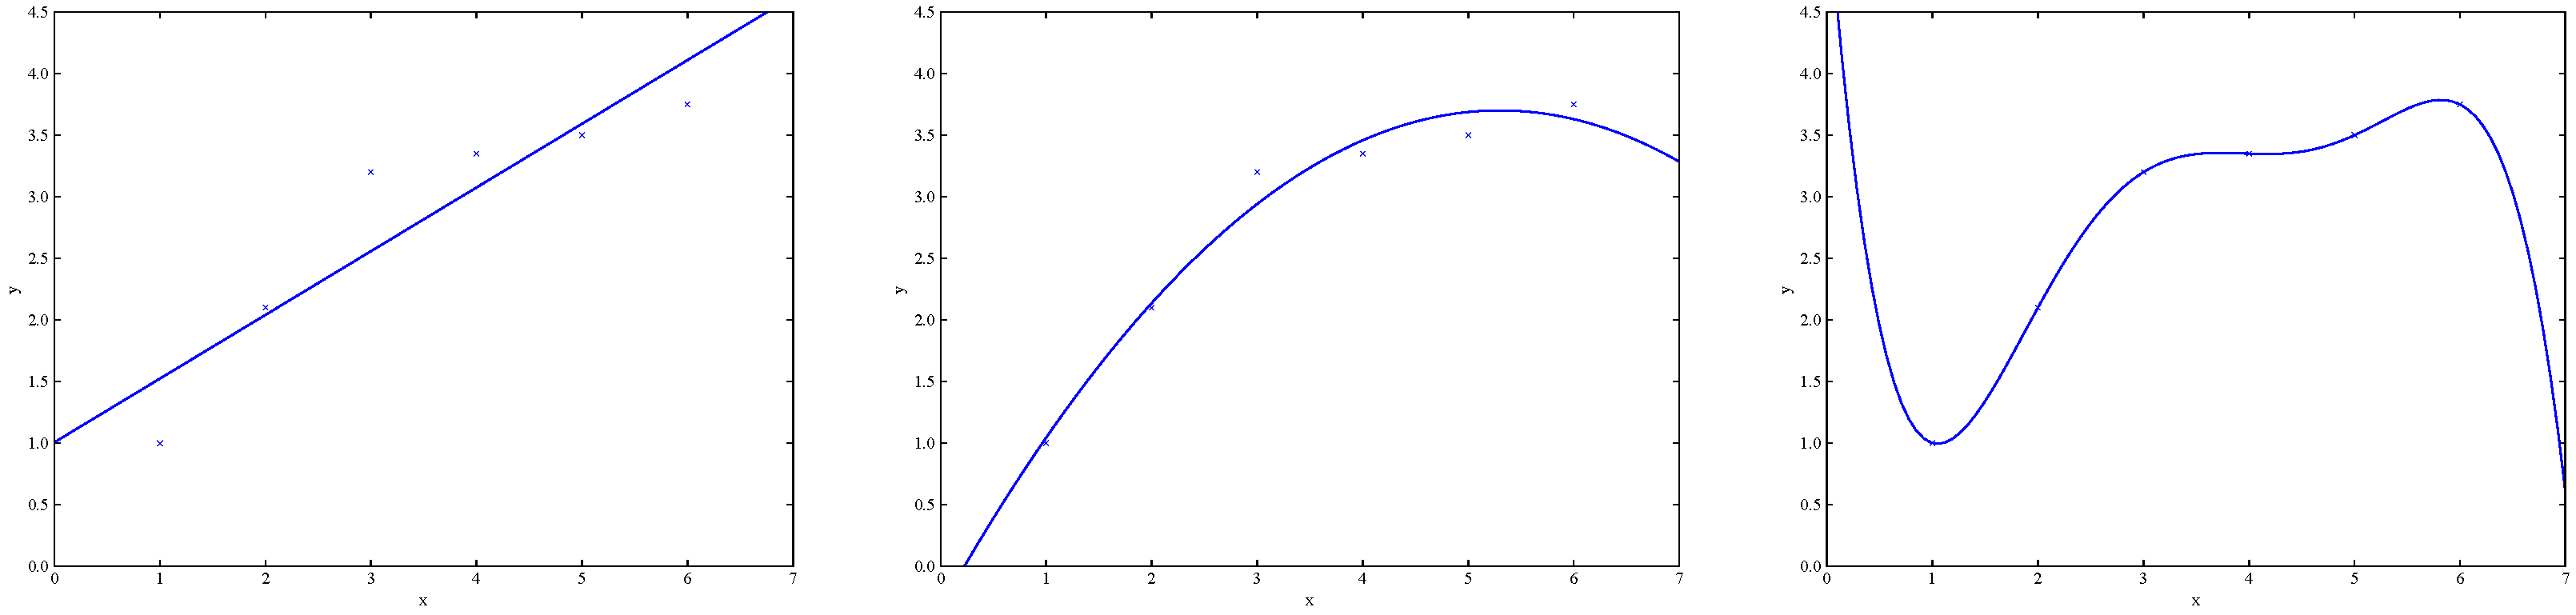
\includegraphics[width=0.93\linewidth]{figs/regression_plot.pdf}
\end{figure}

作为对比,如果我们添加一个额外的特征 $x^2$,然后拟合模型 $y = \theta_0 + \theta_1 x + \theta_2 x^2$,那么对数据的拟合效果可能会有所改善(参见中间图)。有人可能会简单地认为添加的特征越多越好。然而,过度添加特征也存在风险:最右边的图展示了拟合一个五阶多项式 $y = \sum_{j=0}^5 \theta_j x^j$ 的结果。尽管这条拟合曲线完美地穿过了所有数据点,我们也不能期望它能很好地预测不同居住区域 ($x$) 的房价 ($y$)。非正式地借用一下拟合的术语,可以说左边的图是\textbf{欠拟合 (underfitting)} 的一个例子——模型未能捕捉到数据中明显的结构——而右边的图则是一个\textbf{过拟合 (overfitting)} 的例子。(在课程后续的学习理论部分,我们将正式定义这些概念,并更严谨地探讨判断一个假设优劣的标准。)

正如先前讨论的,特征的选择对于确保学习算法的良好性能至关重要。(在后续关于模型选择的讨论中,我们也会介绍一些能够自动选择合适特征的算法。)在本节中,我们将简要介绍局部加权线性回归 (locally weighted linear regression, LWR) 算法。该算法假设有足够的训练数据,使得特征的选择不那么关键。鉴于读者将在作业中自行探索 LWR 算法的一些特性,本节的讲解将较为简略。

在原始的线性回归算法中,为了使用输入 $x$ 进行预测(即计算 $h(x)$ 的值),通常需要执行以下步骤:

\begin{enumerate}
    \item 拟合 $\theta$ 以最小化 $\sum_i (y^{(i)} - \theta^T x^{(i)})^2$。
    \item 输出 $\theta^T x$。
\end{enumerate}

相比之下,局部加权线性回归算法执行以下步骤:

\begin{enumerate}
    \item 拟合 $\theta$ 以最小化 $\sum_i w^{(i)} (y^{(i)} - \theta^T x^{(i)})^2$。
    \item 输出 $\theta^T x$。
\end{enumerate}

这里,$w^{(i)}$ 是非负的\textbf{权重 (weights)}。直观上,对于特定的训练样本 $i$,如果 $w^{(i)}$ 较大,则在确定参数 $\theta$ 时,模型会更倾向于使 $(y^{(i)} - \theta^T x^{(i)})^2$ 误差项尽可能小。反之,如果 $w^{(i)}$ 较小,则该误差项在拟合过程中基本上会被忽略。

一种常用的权重选择方法是\footnote{如果 $x$ 是向量,则推广为 $w^{(i)} = \exp(-(x^{(i)} - x)^T (x^{(i)} - x) / (2\tau^2))$,或者 $w^{(i)} = \exp(-(x^{(i)} - x)^T \Sigma^{-1} (x^{(i)} - x) / (2\tau^2))$,其中 $\tau$ 和 $\Sigma$ 需要选择合适的值。}
\[
    w^{(i)} = \exp\left(-\frac{(x^{(i)} - x)^2}{2\tau^2}\right).
\]
需要注意的是,权重取决于要评估的特定点 $x$。此外,如果 $|x^{(i)} - x|$ 的值很小,则 $w^{(i)}$ 接近 1;如果 $|x^{(i)} - x|$ 的值很大,则 $w^{(i)}$ 会很小。因此,在选择 $\theta$ 时,靠近查询点 $x$ 的训练样本(即其误差项 $y^{(i)} - \theta^T x^{(i)}$)会被赋予更高的“权重”。(另外需要说明的是,尽管权重的表达式形式上类似于高斯分布的概率密度函数,但 $w^{(i)}$ 与高斯分布并没有直接联系,特别是 $w^{(i)}$ 并非随机变量,无论是正态分布还是其他分布。)参数 $\tau$ 控制着训练样本的权重随其与查询点 $x$ 距离衰减的速度;$\tau$ 被称为\textbf{带宽 (bandwidth)} 参数,这也是在作业中需要进行实验的内容。

局部加权线性回归是我们遇到的第一个\textbf{非参数 (non-parametric)} 算法示例。之前讨论的(无权重)线性回归算法被称为\textbf{参数化 (parametric)} 学习算法,因为它通过固定数量的参数($\theta_i$)来拟合数据。一旦这些参数 $\theta_i$ 被确定并存储下来,就不再需要保留训练数据来进行后续的预测。相比之下,为了使用局部加权线性回归进行预测,必须保留整个训练集。术语“非参数”(大致)反映了这样一个事实:表示假设函数 $h$ 所需存储的数据量与训练集的大小呈线性关系。